%% Created by:  H. XU
%% Date:        Oct 27, 2016
%% Email:       78112407@qq.com

%% ========================================================= %%
%%      Note: all the files must be encoded in UTF8          %%
%% ========================================================= %%

\documentclass[a4paper, 11pt, UTF8]{report}

\usepackage[boldfont, CJKnumber]{xeCJK}
%%-----------------------------------------------------%%
%% change the main font
%%\setCJKmainfont[BoldFont=STHeiti, ItalicFont=STKaiti]{FZJSong-Z01S}
\setCJKmainfont[BoldFont=STHeiti, ItalicFont=STKaiti]{STSong}
%%-----------------------------------------------------%%
\setCJKfamilyfont{FangSong}{STFangsong}
\setCJKfamilyfont{HeiTi}{STHeiti}
\setCJKfamilyfont{KaiShu}{STKaiti}
\setCJKfamilyfont{YingBi}{STXingkai}
\setCJKfamilyfont{SongTi}{STSong}
\setCJKfamilyfont{WeiBei}{STXinwei}
\setCJKfamilyfont{ZhongSong}{STZhongsong}
%%-----------------------------------------------------%%
\DeclareRobustCommand{\fangsong}{\CJKfamily{FangSong}}
\DeclareRobustCommand{\heiti}{\CJKfamily{HeiTi}}
\DeclareRobustCommand{\kaiti}{\CJKfamily{KaiShu}}
\DeclareRobustCommand{\songti}{\CJKfamily{SongTi}}
\DeclareRobustCommand{\yingbi}{\CJKfamily{YingBi}}
\DeclareRobustCommand{\weibei}{\CJKfamily{WeiBei}}
\DeclareRobustCommand{\zhongsong}{\CJKfamily{ZhongSong}}
%%-----------------------------------------------------%%

% =================================================================== %
% Adjust the distance of the report
% =================================================================== %

% distance between lines
% 这就是中文的1.5倍
\renewcommand{\baselinestretch}{1.4}

%% distance between paragraph
\parskip 2mm

%% 第一段空两格
\usepackage{indentfirst}

%% 每段段首空格
\parindent 2.4em

%% white, black, red, green, blue, cyan, magenta, yellow, brown
\usepackage[]{color}
\usepackage{xcolor} % Required for specifying colors by name

%% insert picture
\usepackage{graphics}
\graphicspath{ {01Figures/} }

%% insert code
\usepackage{listings}

\lstset{ %
  backgroundcolor = \color{white},   % choose the background color; you must add \usepackage{color} or \usepackage{xcolor}
  basicstyle = \footnotesize\ttfamily,         % the size of the fonts that are used for the code
  breakatwhitespace = false,         % sets if automatic breaks should only happen at whitespace
  breaklines = true,                 % sets automatic line breaking
  captionpos = t,                    % sets the caption-position to bottom
  commentstyle = \color{brown},    % comment style
  deletekeywords = {...},            % if you want to delete keywords from the given language
  escapeinside={\%*}{*)},          % if you want to add LaTeX within your code
  extendedchars=true,              % lets you use non-ASCII characters; for 8-bits encodings only, does not work with UTF-8
  frame =single,	                   % adds a frame around the code
  keepspaces=true,                 % keeps spaces in text, useful for keeping indentation of code (possibly needs columns=flexible)
  keywordstyle=\color{blue},       % keyword style
  language = python,                 % the language of the code
  otherkeywords={*,...},           % if you want to add more keywords to the set
  numbers=left,                    % where to put the line-numbers; possible values are (none, left, right)
  numbersep = 5pt,                   % how far the line-numbers are from the code
  numberstyle=\tiny\color{gray}, % the style that is used for the line-numbers
  rulecolor=\color{black},         % if not set, the frame-color may be changed on line-breaks within not-black text (e.g. comments (green here))
  showspaces=false,                % show spaces everywhere adding particular underscores; it overrides 'showstringspaces'
  showstringspaces=false,          % underline spaces within strings only
  showtabs=false,                  % show tabs within strings adding particular underscores
  stepnumber = 1,                    % the step between two line-numbers. If it's 1, each line will be numbered
  stringstyle=\color{blue},     % string literal style
  tabsize = 4,	                   % sets default tabsize to 4 spaces
  title=\lstname                   % show the filename of files included with \lstinputlisting; also try caption instead of title
}

%% for math
\usepackage{amsmath}
\usepackage{amsfonts}
\usepackage{amssymb}

%% ----------------------------------------------------------- %%
%% main part
%% ----------------------------------------------------------- %%
\setcounter{part}{0}  %% 保证正文的 part chapter 从1 开始计数
\setcounter{chapter}{0}

%% ============================================================ %%


\begin{document}

\title{智能投顾:理论与实践}
\author{
        \sc{Denis Frederic} \\
        \sc{Email}: \tt{78112407$@$qq.com}\\
        \vspace{0.5\textheight} \phantom{phan}}

\maketitle
\newpage
\pagestyle{empty}

\begin{abstract}    
        本文简单回顾智能投顾(Robo-Advisor)的海内外发展情况,
        主要分析该投资方案的算法,
        并以 Python 模拟实现。
\end{abstract}


\tableofcontents
\newpage

\pagestyle{plain}

%% ----------------------------------------------------------- %%
\chapter{介绍}
%% ----------------------------------------------------------- %%


所谓的智能投顾(Robo-Advisor),是指根据现代资产组合管理理论,
利用机器学习等大数据处理技术,
结合投资者的风险承受力与投资偏好,
为其提供定制的资产投资方案。

由于管理费较低(0.20\% 至 0.50\% 左右),资产标的范围广泛,
同时为客户提供避税服务,该业务在美国发展较为迅速。
但该业务在国内基本没有实质发展。

\section{海外发展情况}

2010年,第一家智能投顾公司 Betterment 成立于纽约。
截至2016年10月末,该公司管理的资产规模约 60 亿美元。

目前,规模最大的智能投顾公司是 Vanguard 基金公司,
智能投顾管理规模约 410 亿美元。
但该公司管理的全部基金规模超过 35,000 亿元,
其智能投顾的规模占比仅为 1.17\% 。

结论:

(1)\emph{发展速度较快}。
从 2010 年至 2016 年,
智能投顾公司管理的资产规模从无到有,
到达了 3,000 亿(参见图\ref{fig:adviosr})。

(2)\emph{占比较低}。
全美的基金管理规模是(\textcolor{red}{TODO} 查询),
智能投顾占比是?

\begin{figure}[htbp!]
        \centering
        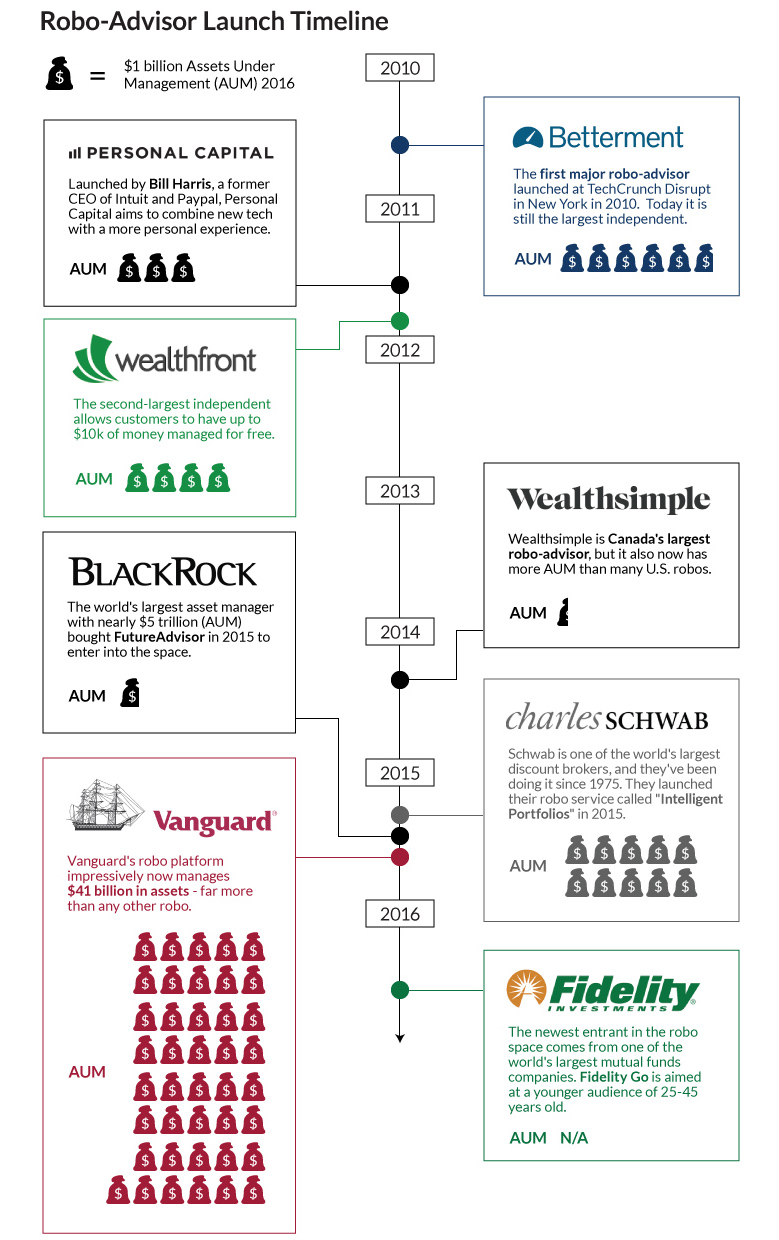
\includegraphics[height=0.9\textheight]{advisor}
        \caption{智能投顾发展一览\newline
                (图片来源:
                \underline{www.visualcapitalist.com/robo-advisor-arms-race})}
        \label{fig:adviosr}
\end{figure}

\section{国内情况}

在目前的法律法规框架下,国内该类业务已被叫停。
此外,国内资产标的范围较小,费用较高,并且没有相关税收优惠政策,
都制约了该类业务的发展。

\subsection{弥财}

国内的弥财(\underline{https://micaiapp.com})
从设计到理念,都比较接近美国的 WealthFront 公司。
该公司的资产标的均为海外资产,并且需要投资者自行换汇。

但经本人测试,9月初该公司申请了账户,到目前还没有开户成功,
并且官方提供的资产电话也无人接听。可能是受到监管的影响,
无法开展业务。

\subsection{蛋卷基金}

国内的雪球网(\textcolor{red}{TODO} 查询)


%% ----------------------------------------------------------- %%
\chapter{实践出真知}
%% ----------------------------------------------------------- %%


本节构建资产组合。
算法的理论基础是资本资产定价模型 CAPM (\textcolor{red}{TODO} 链接),
同时参考 
wealthfront~\footnote{https://research.wealthfront.com/whitepapers/investment-methodology/}
的介绍。
算法主要通过 Python (\textcolor{red}{TODO} 链接)实现,
代码部分参考了通联数据(\textcolor{red}{TODO} 链接),
海外资产的数据由 Yahoo Finance (\textcolor{red}{TODO} 链接)提供,
国内资产的数据由 TuShare (\textcolor{red}{TODO} 链接)提供。

改进的方向:
(1)选取资产
(2)评估资产的相关性
(3)预测资产收益率
(4)模拟不同组合

本文的资产标的主要涵盖股票、黄金、房地产、原油及货币基金。

主要的资产组合都是ETF。
(\textcolor{red}{TODO} 解释为什么要用 etf)
手续费较低,流通性好,可以日内交易。
顺便提一下,\emph{华泰证券}~\footnote{此处不是广告!该券商未以任何形式提供赞助 -\_- }
 ETF 交易费最低 0.1 元!如果用来少量的搭建组合,还是比较划算。
其他券商还是最低 5 元。



\section{ETF 费用一览}

(\textcolor{red}{TODO} 各 etf 的管理费、规模、成立日期,管理人)

国内的 ETF 收费太高,
QDII 组合费用(管理费+托管费)在 1.00\% 左右,
海外的约在 0.10\% 左右。

\section{算法分析} 

假设资产池中有 N 个备选资产。对于资产 $i$ $(1 \le i \le N)$ ,
其年化预期收益率为$\mu_i$,波动率 $\sigma_i$。
全部资产的协方差矩阵为 $V \in \mathbb{R}^{N\times N}$,
其中,$V_{i,j}$ 表示资产 $i$ 与资产 $j$ 的相关性系数。 
特别地 $V^\top = V$,
并且 $V_{k,k} = 1$ $(k=1, \ldots, N)$ 。

给定一个资产组合的权重集:
$\{w = (w_1, \ldots, w_N)^\top \in \mathbb{R}^{N\times 1}
        \;\colon\; \sum^N_{i=1} w_i = 1, w_i \ge 0 \}$,
我们下面计算该集合中对应“有效边界” (Efficient frontier) 对应的子集合。
即:任意给定一个预期收益率 $\mu$
$( \min\{\mu_i\} \le \mu \le \max\{\mu_j\} )$,
我们计算 $\mu$ 对应的全部组合中,
波动率最小的组合
$w(\mu)$~\footnote{表示 $w(\cdot)$ 是一个关于 $\mu$ 的函数}。

该问题等价于如下的一个二次优化问题:
\begin{align*}
        \min \quad & \frac{1}{2} w^\top V w \\
        s.t.\quad  & \sum^N_{i=1} w_i \cdot \mu_i = \mu \\
                   & \sum^N_{i=1} w_i = 1 \\
                   & w_i \ge 0 \;,  \quad (1 \le i \le N) \\
\end{align*}
Python 中 \tt{Cvxopt} 包可以解决该优化问题。

\section{Python Code}
本部分,我们实现上述算法。
代码分为两部分:
(1)根据我们选定的资产,下载其历史数据;
(2)针对每一个资产,估算其年化预期收益率 $\mu_i$、
波动率 $\sigma_i$, 
以及全部资产间的协方差矩阵 $V$。
最后计算全部资产的有效边界(Efficient frontier)。

\subsection{选定资产}

我们选取的国内资产拟定为货币基金ETF,
上证50ETF,中证500ETF,汇深300ETF,
恒生ETF,债券ETF,黄金ETF;
海外资产选取
标普500ETF(SPY),纳斯达克指数(QQQ),
USO,XOP,
黄金ETF(GLD)。

详见代码:

\lstinputlisting[ language=Python,
                  caption = Download the data ]
                {../02PythonCode/01ETFDownloadData.py}


\newpage
\subsection{有效边界}

估算资产的年化预期收益率以、波动率以及相关性系数。

\lstinputlisting[ language=Python,
                  caption = Draw the captial allocation line ]
                {../02PythonCode/02ETFCAL.py}

\end{document}
